% !TeX root = ../main-4.tex
\providecommand{\nextrevision}[1]{#1}
\section{Experiments}\label{sec:experiments}


\subsection{Experimental setup}\label{sec:setup}

\subsubsection{Datasets}\label{sec:datasets}

We evaluate SAKI on five public audio classification datasets: \greenrevision{ESC-50~\cite{piczak2015esc}, UrbanSound8K~\cite{salamon2014urbansound}, TUT Acoustic Scenes 2017 (TUT2017)~\cite{mesaros2016tut,mesaros2017dcase}, FSD50K~\cite{fonseca2022fsd50k}, and AudioSet~\cite{gemmeke2017audioset}}. ESC-50 contains 2,000 five-second clips from 50 environmental sound classes. UrbanSound8K contains 8,732 clips of up to four seconds from 10 urban sound classes. \greenrevision{For TUT2017, we combine 4,680 development and 1,620 evaluation clips, yielding 6,300 ten-second clips from 15 acoustic scene classes.} For FSD50K, we use the 10,231 clips in the official evaluation split and all 200 candidate classes. For AudioSet, we use its 527-class evaluation label space and 17,233 publicly accessible audio files that can be decoded. ESC-50, UrbanSound8K, and TUT2017 are single-label datasets; FSD50K and AudioSet are multilabel datasets.

We use \greenrevision{DCASE17-T4~\cite{mesaros2017dcase}} as a development set. It contains 419 publicly accessible, decodable clips from 17 sound event classes. Development labels are used only to select the fusion weight and the number of relations. These parameters are then fixed for all five test datasets. Test labels are used only to compute evaluation metrics, with no role in training, knowledge retrieval, text generation, or relation selection.






\subsubsection{Comparison methods}\label{sec:comparison-methods}

\greenrevision{The comparison includes the following three methods:}

\begin{enumerate}
    \item \textbf{CLAP}: \redrevision{CLAP serves as the knowledge-free baseline. Its pretrained encoders compute similarities between the input audio and candidate class texts without external knowledge.}
    \item \textbf{iKnow\textsuperscript{\dag}}: \redrevision{Our controlled reimplementation of iKnow-audio serves as the knowledge-enhanced baseline.}
    \item \textbf{SAKI}: Our method comprises AAKV, the Sample-level Relation Selector, and Hierarchical Fusion, as described in Section~\ref{sec:method}.
\end{enumerate}

\bluerevision{The paper describes the inference procedure, but the complete curated relation subset $R_q$ and classification inference implementation are not publicly available~\cite{olvera-etal-2025-iknow}. We therefore evaluate a controlled reimplementation under our common protocol.} It is a controlled reimplementation rather than an exact replication of the original system. The protocol and dataset differences are \redrevision{documented in \ref{app:reproduction}.} All internal comparisons use identical test manifests and evaluation code.

\subsubsection{Implementation details}\label{sec:implementation-details}

We use MS-CLAP 2023 as the audio--text backbone and pretrained RotatE for knowledge graph tail prediction. CLAP and RotatE parameters remain unchanged throughout the experiments. Candidate class labels are lowercased, and underscores are replaced with spaces \redrevision{to standardize class label formatting.}

For consistent internal comparisons, we set $K=5$, $M=3$, and $\lambda=100$ in iKnow\textsuperscript{\dag} and all subsequent ablations. Here, $K$ is the number of classes shortlisted by CLAP, and \redrevision{$M$ is the maximum number of tail entities retained for each class--relation pair.} The controlled reimplementation uses normalized scaled log-sum-exp aggregation to reduce aggregation shifts caused by differences in evidence counts. This setting is retained across the experimental configurations.

We use the AKG constructed by iKnow-audio and its 47 relation types as the common candidate relation pool. For classes mapped to the graph, pretrained RotatE retrieves candidate tails for each class--relation pair offline. AAKV uses Qwen2.5-7B-Instruct with greedy decoding. The generated knowledge texts and their CLAP text embeddings are cached before audio inference.

During online inference, CLAP scores all candidate classes and retains the top $K$. SAKI then selects $N_r$ relations according to Section~\ref{sec:relation-selector-method} and combines their evidence with the original CLAP scores.

We select the fusion weight $\alpha$ and the number of relations $N_r$ by grid search on the DCASE17-T4 development set:
\begin{equation}
\alpha\in\{0.3,0.5,0.7\},\qquad
N_r\in\{1,3,5,10\}.
\end{equation}
Configurations are compared first by development Hit@1 and then, in a tie, by MRR. If both metrics are equal, we select the smaller number of relations. The resulting settings, $\alpha=0.3$ and $N_r=5$, are fixed for all five test datasets.

Audio is resampled to 44.1~kHz and processed into seven-second segments. \greenrevision{Shorter clips are repeated to reach seven seconds. For longer clips, MS-CLAP randomly chooses a starting point and extracts one continuous seven-second segment. A seed derived from the fixed value 42 and each audio path makes this choice reproducible; all methods use the same cached audio representation for each sample.} We run the experiments on a server with three NVIDIA GeForce RTX 4090 D GPUs. The software environment comprises Ubuntu 22.04, Python 3.10.19, PyTorch 2.4.0, CUDA 12.1, MS-CLAP 1.3.4, Transformers 4.57.6, and PyKEEN 1.11.1.



\subsubsection{Evaluation metrics}\label{sec:evaluation-metrics}

We report Hit@$k$ and mean reciprocal rank (MRR). Hit@$k$ is the proportion of samples with at least one ground-truth label among the top $k$ classes; we report Hit@1, Hit@3, and Hit@5. \redrevision{MRR averages the reciprocal rank of the highest-ranked ground-truth label in the complete class ranking.} For multilabel samples, all ground-truth labels are positive, and the highest-ranked positive label determines the reciprocal rank. All metrics are reported as percentages, with higher values indicating better performance.

\bluerevision{For each metric, the mean across the five datasets is the arithmetic mean of the five dataset scores, without weighting by sample count.}

To assess the uncertainty of performance differences, we compute 95\% confidence intervals using 10,000 paired bootstrap resamples of the sample-level predictions. For Hit@1, we also apply two-sided exact McNemar tests to paired correctness outcomes and use Holm adjustment for comparisons across the five datasets.

All reported performance differences are computed from unrounded metric values and rounded to two decimal places for presentation.



\twocolumn[{
\begin{minipage}{\textwidth}
\begin{table}[H]
\centering
\caption{Results (\%) for CLAP, iKnow\textsuperscript{\dag}, and SAKI on five zero-shot audio classification test datasets. Higher is better; bold indicates the highest value for each dataset and metric. \textsuperscript{\dag} denotes our controlled reimplementation of iKnow-audio. All three methods use identical test samples.}
\label{tab:main-results}
\setlength{\tabcolsep}{3.5pt}
\resizebox{\textwidth}{!}{%
\begin{tabular}{l*{15}{c}}
\toprule
\multirow{2}{*}{Metric}
& \multicolumn{3}{c}{ESC-50}
& \multicolumn{3}{c}{UrbanSound8K}
& \multicolumn{3}{c}{FSD50K}
& \multicolumn{3}{c}{AudioSet}
& \multicolumn{3}{c}{TUT2017} \\
\cmidrule(lr){2-4}\cmidrule(lr){5-7}\cmidrule(lr){8-10}\cmidrule(lr){11-13}\cmidrule(lr){14-16}
& CLAP & iKnow\textsuperscript{\dag} & SAKI
& CLAP & iKnow\textsuperscript{\dag} & SAKI
& CLAP & iKnow\textsuperscript{\dag} & SAKI
& CLAP & iKnow\textsuperscript{\dag} & SAKI
& CLAP & iKnow\textsuperscript{\dag} & SAKI \\
\midrule
Hit@1
& 91.10 & 91.75 & \textbf{94.25}
& 83.76 & 84.88 & \textbf{87.17}
& 57.35 & 59.84 & \methodrevision{\textbf{64.46}}
& 28.65 & 29.22 & \methodrevision{\textbf{31.29}}
& 40.65 & 44.14 & \textbf{56.87} \\
Hit@3
& 96.75 & \textbf{97.05} & 96.80
& 96.60 & 96.77 & \textbf{96.90}
& 79.65 & \textbf{80.73} & \methodrevision{80.52}
& 46.36 & \textbf{47.04} & \methodrevision{46.90}
& 76.59 & 79.89 & \textbf{80.54} \\
Hit@5
& \textbf{97.65} & \textbf{97.65} & \textbf{97.65}
& \textbf{98.65} & \textbf{98.65} & \textbf{98.65}
& 86.35 & \textbf{86.51} & \methodrevision{86.48}
& 54.80 & \textbf{54.87} & \methodrevision{54.80}
& 92.24 & \textbf{92.68} & 91.79 \\
MRR
& 94.11 & 94.57 & \textbf{95.75}
& 90.40 & 91.08 & \textbf{92.22}
& 70.17 & 71.80 & \methodrevision{\textbf{74.13}}
& 41.06 & 41.54 & \methodrevision{\textbf{42.56}}
& 60.79 & 64.04 & \textbf{70.73} \\
\bottomrule
\end{tabular}
}

\end{table}
\vspace{8pt}
\begin{table}[H]
\centering
\caption{Component ablations (\%, Hit@1/MRR). The plus sign denotes a component added to iKnow\textsuperscript{\dag}. \greenrevision{The mean across the five datasets is the unweighted arithmetic mean of their metrics.} Fusion and Selector abbreviate Hierarchical Fusion and Sample-level Relation Selector. Bold indicates the highest value in each column.}
\label{tab:factorial-ablation}
\setlength{\tabcolsep}{2.5pt}
\resizebox{\textwidth}{!}{%
\begin{tabular}{l*{12}{c}}
\toprule
\multirow{2}{*}{Method}
& \multicolumn{2}{c}{ESC-50}
& \multicolumn{2}{c}{UrbanSound8K}
& \multicolumn{2}{c}{FSD50K}
& \multicolumn{2}{c}{AudioSet}
& \multicolumn{2}{c}{TUT2017}
& \multicolumn{2}{c}{\greenrevision{Mean (5 datasets)}} \\
\cmidrule(lr){2-3}\cmidrule(lr){4-5}\cmidrule(lr){6-7}\cmidrule(lr){8-9}\cmidrule(lr){10-11}\cmidrule(lr){12-13}
& Hit@1 & MRR & Hit@1 & MRR & Hit@1 & MRR & Hit@1 & MRR & Hit@1 & MRR & Hit@1 & MRR \\
\midrule
iKnow\textsuperscript{\dag}
& 91.75 & 94.57 & 84.88 & 91.08 & 59.84 & 71.80 & 29.22 & 41.54 & 44.14 & 64.04 & 61.97 & 72.61 \\
+ AAKV
& 88.65 & 92.63 & 84.52 & 90.59 & 61.60 & 72.65 & 28.65 & 41.16 & 48.68 & 66.20 & 62.42 & 72.65 \\
+ Fusion
& 92.85 & 95.15 & 85.02 & 91.18 & 60.83 & 72.49 & 29.64 & 41.88 & 46.86 & 65.86 & 63.04 & 73.31 \\
+ Selector
& 93.85 & 95.63 & 85.83 & 91.44 & 60.29 & 71.88 & 29.87 & 41.77 & 46.56 & 65.39 & 63.28 & 73.22 \\
+ AAKV + Fusion
& 92.70 & 95.09 & 85.78 & 91.47 & 62.71 & 73.47 & 29.75 & 41.88 & 51.29 & 67.99 & 64.44 & 73.98 \\
+ AAKV + Selector
& 92.85 & 94.90 & 86.96 & 91.86 & \methodrevision{\textbf{64.49}} & \methodrevision{74.02} & \methodrevision{31.23} & \methodrevision{42.46} & 53.54 & 68.80 & \methodrevision{65.81} & \methodrevision{74.41} \\
+ Fusion + Selector
& 93.90 & 95.63 & 85.73 & 91.40 & 60.60 & 71.82 & 30.03 & 41.78 & 47.87 & 65.93 & 63.63 & 73.31 \\
\textbf{SAKI}
& \textbf{94.25} & \textbf{95.75}
& \textbf{87.17} & \textbf{92.22}
& \methodrevision{64.46} & \methodrevision{\textbf{74.13}}
& \methodrevision{\textbf{31.29}} & \methodrevision{\textbf{42.56}}
& \textbf{56.87} & \textbf{70.73}
& \methodrevision{\textbf{66.81}} & \textbf{75.08} \\
\bottomrule
\end{tabular}
}

\end{table}
\end{minipage}
}]

\subsection{Overall results}\label{sec:overall-results}

Table~\ref{tab:main-results} shows that SAKI achieved the highest Hit@1 and MRR among the three methods on all five test datasets. Relative to iKnow\textsuperscript{\dag}, Hit@1 increased by 2.08--12.73 percentage points and MRR by 1.02--6.68 percentage points. iKnow\textsuperscript{\dag} also improved both metrics over CLAP. Under this protocol, graph augmentation and SAKI's approach to organizing knowledge each provided classification gains.

These findings are consistent with iKnow-audio's use of graph knowledge to improve CLAP predictions~\cite{olvera-etal-2025-iknow}. \redrevision{Under the common evaluation protocol, the results for iKnow\textsuperscript{\dag} support the value of class-related knowledge. SAKI achieves further gains over iKnow\textsuperscript{\dag}.} The additional improvement indicates that how knowledge enters classification also matters. Both methods use the same CLAP model and graph resources. Their performance difference therefore reflects the combined effects of knowledge selection, verbalization, and fusion under the evaluated inference configurations.

The gains primarily concern top-1 classification and ground-truth label ranking. On TUT2017, Hit@1 increased from 44.14\% to 56.87\%, and MRR increased from 64.04\% to 70.73\%. Hit@5, however, decreased from 92.68\% to 91.79\%. \greenrevision{Thus, more TUT2017 samples had the correct class at rank one, although slightly fewer had it among the top five.}

Changes in Hit@3 and Hit@5 were smaller on the remaining datasets. Hit@5 matched iKnow\textsuperscript{\dag} on ESC-50 and UrbanSound8K, while both coverage metrics decreased slightly on FSD50K and AudioSet. \greenrevision{Relative to iKnow\textsuperscript{\dag}, SAKI's main gains were in Hit@1 and MRR. Hit@3 and Hit@5 varied across datasets but remained close to those of iKnow\textsuperscript{\dag} overall.}




\subsection{Ablation and component analysis}\label{sec:ablation}
We use component ablations, relation selection controls, and knowledge verbalization controls to examine combined gains, selection strategies, and text representations, respectively. All experiments use the same CLAP model, knowledge graph, candidate classes, class-to-entity mapping, and knowledge retrieval settings.





\subsubsection{Overall ablation}\label{sec:overall-ablation}


Table~\ref{tab:factorial-ablation} compares individual components, \greenrevision{pairs of components}, and SAKI against iKnow\textsuperscript{\dag}. Supplementary Hit@3 and Hit@5 results are provided in Table~\ref{tab:ablation-topk}.

\redrevision{Relation selection and Hierarchical Fusion each improved Hit@1 over iKnow\textsuperscript{\dag} on all five datasets when added individually.} Their respective gains in the unweighted mean Hit@1 were 1.31 and 1.07 percentage points. AAKV alone improved Hit@1 on FSD50K and TUT2017 but reduced it on the other three datasets. Its mean MRR gain was only 0.04 percentage points. The effect of rewriting knowledge text therefore varies across datasets and warrants examination alongside the other components.

\twocolumn[{
\begin{minipage}{\textwidth}
\begin{table}[H]
\centering
\caption{Relation selection strategies with AAKV and Hierarchical Fusion fixed (\%, Hit@1/MRR). \greenrevision{FrozenRq uses the fixed relation set reconstructed for each dataset in our iKnow\textsuperscript{\dag} reimplementation.} Random Top-5 reports the mean over seeds 42, 43, and 44. Bold indicates the highest value in each column.}
\label{tab:relation-selection}
\setlength{\tabcolsep}{2.8pt}
\resizebox{\textwidth}{!}{%
\begin{tabular}{l*{12}{c}}
\toprule
\multirow{2}{*}{Method}
& \multicolumn{2}{c}{ESC-50}
& \multicolumn{2}{c}{UrbanSound8K}
& \multicolumn{2}{c}{FSD50K}
& \multicolumn{2}{c}{AudioSet}
& \multicolumn{2}{c}{TUT2017}
& \multicolumn{2}{c}{\greenrevision{Mean (5 datasets)}} \\
\cmidrule(lr){2-3}\cmidrule(lr){4-5}\cmidrule(lr){6-7}\cmidrule(lr){8-9}\cmidrule(lr){10-11}\cmidrule(lr){12-13}
& Hit@1 & MRR & Hit@1 & MRR & Hit@1 & MRR & Hit@1 & MRR & Hit@1 & MRR & Hit@1 & MRR \\
\midrule
FrozenRq
& 92.70 & 95.09 & 85.78 & 91.47 & \methodrevision{62.71} & \methodrevision{73.47} & \methodrevision{29.75} & \methodrevision{41.88} & 51.29 & 67.99 & \methodrevision{64.44} & \methodrevision{73.98} \\
Frequency Top-5
& 92.85 & 95.23 & 85.10 & 91.04 & \methodrevision{62.66} & \methodrevision{73.30} & \methodrevision{30.10} & \methodrevision{42.14} & 50.54 & 67.40 & \methodrevision{64.25} & \methodrevision{73.82} \\
Random Top-5
& 92.45 & 94.90 & 86.02 & 91.61 & \methodrevision{63.33} & \methodrevision{73.67} & \methodrevision{29.86} & \methodrevision{41.94} & 52.10 & 68.54 & \methodrevision{64.75} & \methodrevision{74.13} \\
\textbf{Sample-level Relation Selector}
& \textbf{94.25} & \textbf{95.75}
& \textbf{87.17} & \textbf{92.22}
& \methodrevision{\textbf{64.46}} & \methodrevision{\textbf{74.13}}
& \methodrevision{\textbf{31.29}} & \methodrevision{\textbf{42.56}}
& \textbf{56.87} & \textbf{70.73}
& \methodrevision{\textbf{66.81}} & \textbf{75.08} \\
\bottomrule
\end{tabular}
}

\end{table}
\end{minipage}
}]

Removing one component from SAKI isolates its contribution when the other two remain enabled. Without AAKV, the unweighted mean Hit@1 and MRR were 63.63\% and 73.31\%; without relation selection, they were 64.44\% and 73.98\%. Removing Hierarchical Fusion yielded 65.81\% and 74.41\%, compared with SAKI's 66.81\% and 75.08\%. \greenrevision{Among the three component pairs, AAKV with relation selection achieved the highest mean Hit@1 and MRR. Adding Hierarchical Fusion increased both means further.} These comparisons support the contribution of each component within the combined configuration. Together with the \greenrevision{results for individual components}, they show that AAKV's gains depend particularly on its use with the other components.

FSD50K provides an exception to this overall trend. Adding Hierarchical Fusion to AAKV with relation selection changed Hit@1 from 64.49\% to 64.46\%, while MRR increased from 74.02\% to 74.13\%. \redrevision{Adding Hierarchical Fusion slightly increased MRR, while Hit@1 remained nearly unchanged.} Combined gains should therefore be assessed using both the unweighted means and individual dataset metrics.

The three components act on successive stages of the scoring process. AAKV changes knowledge texts and their audio--text similarity scores, which also inform relation-specific predictions, relation selection, and final score fusion. The same verbalization method can consequently yield different gains across component configurations, consistent with the contrast between AAKV alone and its combined use. Hierarchical Fusion separates evidence aggregation within each class from the weight assigned to the original CLAP score. Knowledge scores thus influence reranking through an explicit weight.






\subsubsection{Relation selection analysis}\label{sec:relation-analysis}




The component ablations examined the contribution of relation selection. Here, we compare fixed, frequent, and random relation sets with \greenrevision{relation sets selected for each audio sample} under identical knowledge representation and fusion settings. This comparison tests how the strategy for determining relations affects classification.

\greenrevision{FrozenRq uses the fixed relation set reconstructed for each dataset in our iKnow\textsuperscript{\dag} reimplementation. All audio samples in a dataset use that same set.} Frequency Top-5 selects five relations by their counts of class--tail evidence entries in the offline cache. Random Top-5 selects five relations for each audio sample and reports the mean over three fixed seeds. The Sample-level Relation Selector selects five relations using the top-1 voting consensus and \redrevision{top-two score gaps computed separately for each relation for the current audio.}

As shown in Table~\ref{tab:relation-selection}, sample-level relation selection outperformed all three controls in Hit@1 and MRR on every test dataset. Its unweighted mean Hit@1 and MRR were 66.81\% and 75.08\%, exceeding FrozenRq by 2.37 and 1.10 percentage points. The corresponding gains on TUT2017 were 5.59 and 2.73 percentage points. With knowledge texts and fusion rules fixed, this comparison supports selecting relations according to the current audio.

Frequency Top-5 retained the same number of relations as sample-level selection but achieved lower Hit@1 and MRR on all five datasets. \redrevision{Random Top-5 also varied relation sets across samples. Its mean Hit@1 and MRR were 2.06 and 0.95 percentage points lower than those of SAKI.} \greenrevision{At a fixed relation count, selection based on the current audio performed better than selection by cached evidence counts or random assignment.}

\greenrevision{iKnow-audio retrieves class-related tail entities through a curated subset of informative relations~\cite{olvera-etal-2025-iknow}.} SAKI additionally ranks relations using the predictions obtained from their evidence for the current audio. Graph scores and audio predictions serve different purposes: the former measure triple plausibility, whereas the latter reflect the class ranking obtained using each relation's evidence. Top-1 voting prioritizes relations supporting the consensus class; top-two score gaps then distinguish relations within each group. \greenrevision{Both criteria are computed from predictions for the current audio.} \bluerevision{Table~\ref{tab:relation-selection} supports the effectiveness of the combined relation selection strategy.}

\bluerevision{We also examine the relation sets selected for individual audio samples.} The five datasets produced between 1,708 and 15,733 distinct top-5 relation sets, \redrevision{with the most frequent set accounting for 1.06\%--1.53\% of samples.} \bluerevision{These statistics show that the selected relation sets vary across audio samples.} The controlled comparison in Table~\ref{tab:relation-selection} supports the classification benefit of sample-level relation selection. \redrevision{\ref{app:selector-behavior} reports dataset-specific statistics and mean Jaccard overlap with FrozenRq.}
% Author-deferred experiment: voting-only and score-gap-only controls may be added after their results are available. Not included in Limitations.





\begin{figure*}[!t]
\begin{minipage}{\textwidth}
\begin{table}[H]
\centering
\caption{Knowledge text representations (\%, Hit@1/MRR). All three use the same relation selection algorithm and Hierarchical Fusion settings. Bold indicates the highest value in each column.}
\label{tab:knowledge-verbalization}
\setlength{\tabcolsep}{3.2pt}
\resizebox{\textwidth}{!}{%
\begin{tabular}{l*{12}{c}}
\toprule
\multirow{2}{*}{Method}
& \multicolumn{2}{c}{ESC-50}
& \multicolumn{2}{c}{UrbanSound8K}
& \multicolumn{2}{c}{FSD50K}
& \multicolumn{2}{c}{AudioSet}
& \multicolumn{2}{c}{TUT2017}
& \multicolumn{2}{c}{\greenrevision{Mean (5 datasets)}} \\
\cmidrule(lr){2-3}\cmidrule(lr){4-5}\cmidrule(lr){6-7}\cmidrule(lr){8-9}\cmidrule(lr){10-11}\cmidrule(lr){12-13}
& Hit@1 & MRR & Hit@1 & MRR & Hit@1 & MRR & Hit@1 & MRR & Hit@1 & MRR & Hit@1 & MRR \\
\midrule
Direct concatenation
& 93.90 & 95.63 & 85.73 & 91.40 & 60.60 & 71.82 & 30.03 & 41.78 & 47.87 & \methodrevision{65.93} & 63.63 & 73.31 \\
Raw triple
& 94.10 & \textbf{95.77} & 86.43 & 91.79 & 59.58 & 71.00 & 29.25 & 41.01 & 47.95 & 64.97 & 63.46 & 72.91 \\
\textbf{AAKV}
& \textbf{94.25} & 95.75
& \textbf{87.17} & \textbf{92.22}
& \methodrevision{\textbf{64.46}} & \methodrevision{\textbf{74.13}}
& \methodrevision{\textbf{31.29}} & \methodrevision{\textbf{42.56}}
& \textbf{56.87} & \textbf{70.73}
& \methodrevision{\textbf{66.81}} & \textbf{75.08} \\
\bottomrule
\end{tabular}
}
\end{table}
\vspace{8pt}
\begin{figure}[H]
    \centering
    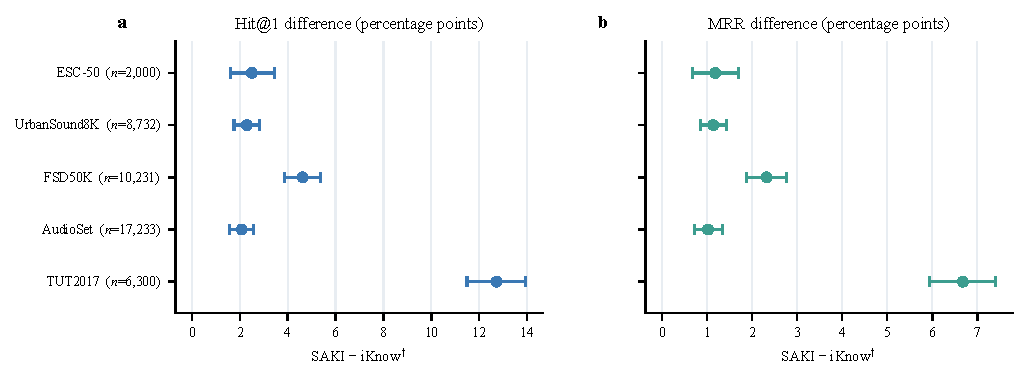
\includegraphics[width=0.80\textwidth]{figures/further_analysis/fig_statistical_significance.pdf}
    \caption{Paired Hit@1 and MRR differences between SAKI and iKnow\textsuperscript{\dag}, with 95\% confidence intervals. Points denote observed differences; error bars are obtained from 10,000 paired bootstrap resamples of test audio. The vertical dashed line marks zero difference. The horizontal axis is in percentage points.}
    \label{fig:statistical-significance}
\end{figure}
\end{minipage}
\end{figure*}

\subsubsection{Knowledge verbalization analysis}\label{sec:verbalization-analysis}


We compare three knowledge text representations under the same relation selection algorithm and Hierarchical Fusion rules. Direct concatenation joins class names and tail entities; Raw triple retains the class, relation, and tail fields. AAKV organizes triples into sound descriptions that preserve entity and relation semantics. Each configuration computes relation-specific class scores from its own texts, allowing representation choices to be compared within the same inference procedure.

Table~\ref{tab:knowledge-verbalization} shows that AAKV achieved higher Hit@1 than both controls on all five datasets. Its unweighted mean Hit@1 and MRR reached 66.81\% and 75.08\%, exceeding Direct concatenation by 3.18 and 1.77 percentage points. Raw triple yielded mean Hit@1 and MRR of 63.46\% and 72.91\%, slightly below Direct concatenation's 63.63\% and 73.31\%. Simply adding relation fields thus provided limited benefit in this experiment, suggesting that their textual organization also matters.

ReCLAP expands class semantics through acoustic descriptions and prompts covering diverse scenes, and reports improved zero-shot classification with prompt augmentation~\cite{ghosh2024reclap}. Our verbalization comparison likewise supports the importance of text representation, although AAKV specifically expresses existing triple relations as constrained sound descriptions. Natural-language sentences explicitly connect the class, relation, and tail entity, providing CLAP's text encoder with a coherent semantic expression. This may help explain AAKV's gains over \greenrevision{text consisting of separate triple fields}.

\bluerevision{Relative to Direct concatenation, AAKV increased Hit@1 by 3.86 percentage points on FSD50K and 9.00 on TUT2017, compared with 0.35 on ESC-50. On ESC-50, its MRR was comparable to Raw triple (95.75\% versus 95.77\%).}



\subsection{Further analysis}\label{sec:further-analysis}

We examine uncertainty in performance differences, sample-level prediction transitions, parameter selection, and computational cost.



\subsubsection{Statistical significance}\label{sec:statistics}

\redrevision{We assess uncertainty in the Hit@1 and MRR gains of SAKI over iKnow\textsuperscript{\dag} using paired bootstrap confidence intervals.} Following the paired bootstrap procedure in Section~\ref{sec:evaluation-metrics}, we use the same resampled audio indices for both methods. The 2.5th and 97.5th percentiles of the difference distribution define the 95\% confidence interval.

In Figure~\ref{fig:statistical-significance}, all observed Hit@1 and MRR differences are positive, and their 95\% confidence intervals lie entirely above zero. TUT2017 shows the largest Hit@1 gain, at 12.73 percentage points, with a confidence interval of [11.49, 13.95] percentage points. The intervals on the other datasets also exclude zero, supporting the observed gains under resampling of the current test audio.

\bluerevision{These intervals reflect uncertainty from resampling test samples, with the models and inference settings held fixed.}


\subsubsection{\nextrevision{Prediction transitions and case study}}\label{sec:cases}

\redrevision{Transitions from incorrect iKnow\textsuperscript{\dag} predictions to correct SAKI predictions outnumbered the reverse transitions on all five datasets. The difference yielded a net improvement in top-1 accuracy.} On FSD50K, for example, 991 incorrect predictions became correct, while 518 correct predictions became incorrect. Reranking therefore corrected errors while also changing some originally correct decisions. The gains in the main table summarize the net effect of both changes.

\begin{figure}[H]
    \centering
    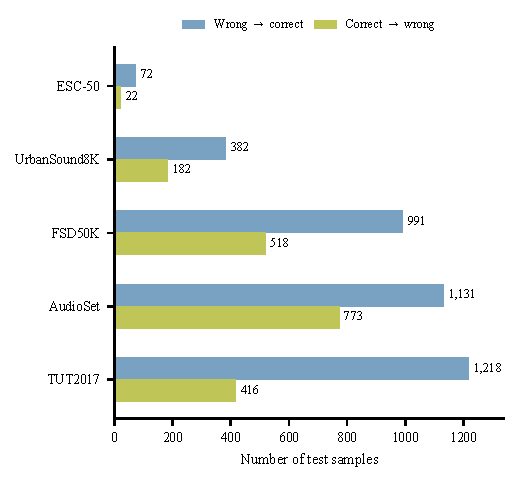
\includegraphics[width=0.84\columnwidth]{figures/further_analysis/fig_prediction_transitions.pdf}
    \caption{Sample-level Hit@1 transitions from iKnow\textsuperscript{\dag} to SAKI. Blue bars count \greenrevision{transitions from incorrect to correct predictions}; yellow-green bars count \greenrevision{transitions from correct to incorrect predictions}. Their difference is the net increase in correct predictions with SAKI.}
    \label{fig:prediction-transitions}
\end{figure}

Figure~\ref{fig:prediction-transitions} decomposes the overall Hit@1 gains into error corrections and prediction degradations.

We applied two-sided exact McNemar tests to the discordant pairs shown in the figure. All five $p$ values remained below 0.05 after Holm adjustment, with a maximum of approximately $2.26\times10^{-7}$ (Table~\ref{tab:mcnemar-tests}). Together with the transition directions, these results support SAKI's Hit@1 advantage after controlling the familywise error rate across the five tests.

Table~\ref{tab:case-study} illustrates three types of ranking changes. In the correction case, \textit{wind} moved from fifth to first. In the \greenrevision{case of improved ranking}, \textit{sea waves} rose from third to second, while SAKI predicted \textit{frog} at rank one. In the degradation case, \textit{washing machine} fell from first to fourth, and SAKI instead predicted \textit{engine}.

\begin{table}[H]

\centering

\caption{Three representative prediction changes on ESC-50. Parentheses give the ground-truth class rank. \redrevision{The cached evidence texts are reproduced verbatim and provide examples of evidence read for candidate classes during inference.} They do not establish the independent contribution of an individual evidence item to the prediction change.}

\label{tab:case-study}

\footnotesize

\setlength{\tabcolsep}{2pt}

\begin{tabular*}{\columnwidth}{@{\extracolsep{\fill}}llll@{}}

\toprule

Case & True class & iKnow\textsuperscript{\dag} & SAKI \\

\midrule

Correction
& wind & train (5) & wind (1) \\

\multicolumn{4}{@{}p{\columnwidth}@{}}
{\textit{AAKV evidence: The sound of wind is instance of ocean.}} \\

\addlinespace[2pt]

Rank improvement
& sea waves & crickets (3) & frog (2) \\

\multicolumn{4}{@{}p{\columnwidth}@{}}
{\textit{AAKV evidence: The sound of frog is part of a wetland scene.}} \\

\addlinespace[2pt]

Degradation
& washing machine & washing machine (1) & engine (4) \\

\multicolumn{4}{@{}p{\columnwidth}@{}}
{\textit{AAKV evidence: The sound of engine is instance of motorcycle.}} \\

\bottomrule

\end{tabular*}

\end{table}

These cases illustrate how Hit@1 and MRR capture different ranking changes. Moving \textit{wind} to first improves both metrics. For \textit{sea waves}, reciprocal rank increases from $1/3$ to $1/2$, while Hit@1 remains zero. Moving \textit{washing machine} away from first reduces both metrics. Reporting Hit@1 and MRR together thus distinguishes error correction, rank improvement below first place, and prediction degradation.

Prediction degradation also highlights the limits of relation consensus. \redrevision{Class scores for all relations are computed using the same CLAP encoder. Agreement among their top-1 predictions may therefore reflect matching biases shared by the underlying model.} Consensus and larger top-two score gaps provide selection criteria, but do not establish evidence correctness or relevance to the sample.

\Needspace{8\baselineskip}
\subsubsection{Parameter sensitivity}\label{sec:parameters}

We examine the fusion weight $\alpha$ and relation count $N_r$ on the DCASE17-T4 development set. The search range and selection rule are given in Section~\ref{sec:implementation-details}.

\begin{figure}[H]
    \centering
    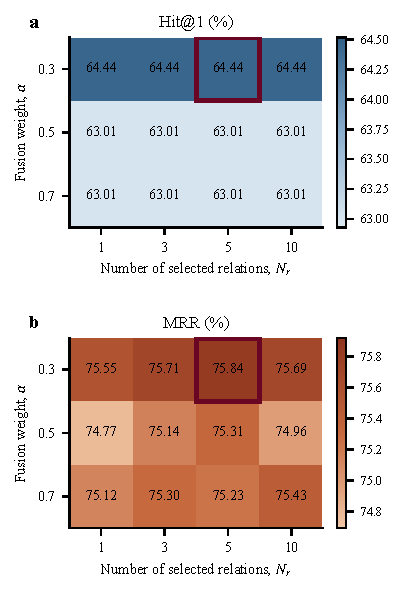
\includegraphics[width=0.80\columnwidth]{figures/further_analysis/fig_parameter_sensitivity.pdf}
    \caption{Parameter sensitivity on the DCASE17-T4 development set. (a) Hit@1 for different fusion weights $\alpha$ and relation counts $N_r$. (b) MRR for the same configurations. The outlined configuration, $\alpha=0.3$ and $N_r=5$, is selected by maximizing Hit@1 and then MRR.}
    \label{fig:parameter-sensitivity}
\end{figure}

Figure~\ref{fig:parameter-sensitivity}(a) shows identical Hit@1 for all four relation counts at each fixed $\alpha$. Hit@1 was 64.44\% at $\alpha=0.3$, compared with 63.01\% at $\alpha=0.5$ or $0.7$. Within this search range, top-1 accuracy varied with the fusion weight but remained unchanged across relation counts.

MRR distinguishes configurations with identical Hit@1 (Figure~\ref{fig:parameter-sensitivity}(b)). At $\alpha=0.3$, increasing $N_r$ from one to five raised MRR from 75.55\% to 75.84\%; increasing it to ten reduced MRR to 75.69\%. \redrevision{The benefit of adding relations was therefore nonmonotonic within the tested range.} Following the \greenrevision{predefined rule for choosing parameters on the development set}, we selected $\alpha=0.3$ and $N_r=5$ and fixed them for all five test datasets.


\Needspace{30\baselineskip}
\subsubsection{Computational cost analysis}\label{sec:computational-cost}
\begin{table}[!t]
\centering
\caption{Online inference efficiency and offline cache size at batch size 1. Latency, peak GPU memory, and cache size are unweighted means across the five test datasets. Relative overhead is the ratio to mean CLAP latency; throughput is computed from mean latency.}
\label{tab:computational-cost}
\small
\setlength{\tabcolsep}{4pt}
\begin{tabular}{lccc}
\toprule
Metric & CLAP & iKnow\textsuperscript{\dag} & SAKI \\
\midrule
Latency (ms/sample) & 24.37 & 25.16 & 86.52 \\
Relative overhead & 1.00$\times$ & 1.03$\times$ & 3.55$\times$ \\
Throughput (samples/s) & 41.03 & 39.74 & 11.56 \\
Peak GPU memory usage (MiB) & 693.60 & 700.30 & 743.22 \\
Offline cache (MiB) & 0.63 & 6.74 & 50.52 \\
\bottomrule
\end{tabular}
\end{table}

We compare the three methods on identical hardware and test samples. \redrevision{For each dataset, we selected 200 fixed samples and processed 20 samples for warm-up. We then repeated timing five times at batch size one.} Online time includes audio preprocessing, CLAP audio encoding, scoring, and ranking. RotatE retrieval, AAKV generation, and text encoding are performed offline. Table~\ref{tab:computational-cost} reports unweighted mean latency, peak GPU memory usage, and cache size across the five datasets. Relative overhead and throughput are calculated from mean latency. The cache includes text embeddings and evidence index mappings, excluding model weights, raw audio, and the source knowledge graph.



Table~\ref{tab:computational-cost} shows that iKnow\textsuperscript{\dag}'s latency of 25.16~ms/sample was close to CLAP's 24.37~ms/sample. SAKI required 86.52~ms/sample, corresponding to 3.55 times CLAP's latency and a throughput of 11.56 samples/s. Peak GPU memory usage was 743.22~MiB for SAKI and 693.60~MiB for CLAP; offline caches were 50.52 and 0.63~MiB, respectively. \redrevision{Relative to CLAP, SAKI showed a smaller proportional increase in peak GPU memory usage than in latency, while its cache size increased substantially.} In these measurements, deployment costs mainly involved longer online processing and greater storage for precomputed evidence. \greenrevision{SAKI also performs relation-specific scoring, relation ranking, and evidence fusion online, consistent with its higher measured latency.}

\subsection{Limitations}\label{sec:limitations}

SAKI's applicability depends on both knowledge quality and the underlying model. AAKV constrains how triples are expressed, while retrieval errors and associations irrelevant to the current audio can still enter the classification evidence. The current evaluation uses fixed MS-CLAP 2023 and RotatE models and 47 candidate relations. The observed gains apply to these resources and the five test datasets; transfer to other audio--language models and knowledge graphs requires further evaluation.

Online relation evaluation also increases inference time and cache requirements, limiting the flexibility of the current implementation in low-latency settings. Future work can assess evidence reliability to reduce unsuitable knowledge and use lightweight relation preselection to reduce the number of evaluated relations. These directions seek a more favorable balance between classification performance and inference cost.


\FloatBarrier
